\chapter{Návrh uživatelského rozhraní}

Návrh uživatelského rozhraní vychází z analýzy konkurenčních webů probíraných v sekci \ref{analyza} a z požadavků na aplikaci ze sekce \ref{requirements}. Zaměřím se na návrh těchto stránek:
\begin{itemize}
    \item Celkové rozvržení webu
	\item Hlavní stránka
	\item Detail nabídky
	\item Můj profil
	\item Profil uživatele
	\item Nová nabídka
	\item Ostatní sekce
\end{itemize}
Dále se zaměřím na návrh dalších částí jako je:
\begin{itemize}
    \item Hodnocení uživatelů
	\item Řazení výpisu nabídek
	\item Změna adresy uživatele
\end{itemize}
V současné době stále stoupá procento přístupů na web z mobilních zařízení, a proto se při návrhu uživatelského rozhraní budu soustředit nejen na verzi pro počítače s vysokým rozlišením, ale také na verzi určenou pro mobilní zařízení.

\section{Celkové rozvržení webu}

\label{nur:layout}

Každá nabídka disponuje svou polohou a poloměrem, ve kterém je uživatel ochoten směnit své peníze. V~takové situaci je vhodné použít mapu. Mapa se však nehodí pro všechny podstránky aplikace. Proto byla navržena dvě různá rozložení webu -- s~mapou a bez mapy.

\subsection{Rozvržení webu s~mapou}
Velmi povedené rozvržení stránky lze pozorovat na webu Sreality.cz, analyzovaného v~kapitole \ref{analyza:sreality}, čímž je také inspirován tento návrh. Polovinu stránky při tomto rozvržení zabírá mapa a druhou polovinu textová část. Toto rozvržení lze vidět na obrázku \ref{fig:tur:homepage}.

Textová část stránky obsahuje vedle hlavního obsahu hlavičku, kde se nachází logo a hlavní menu, dále pak patičku s~odkazy na informační stránky aplikace.

\subsection{Rozvržení webu bez mapy}
V~podstatě se jedná o~totožné rozvržení s~tím rozdílem, že zde je mapa vynechána. Rozvržení lze vidět na obrázku \ref{fig:tur:offer-detail-no-map} na straně \pageref{fig:tur:offer-detail-no-map}.
\section{Hlavní stránka}

\label{nur:homepage}
Stránka používá rozvržení webu s~mapou. Podobu stránky lze vidět na obrázku \ref{fig:tur:homepage}.

\begin{figure}[!h]
    \centering
    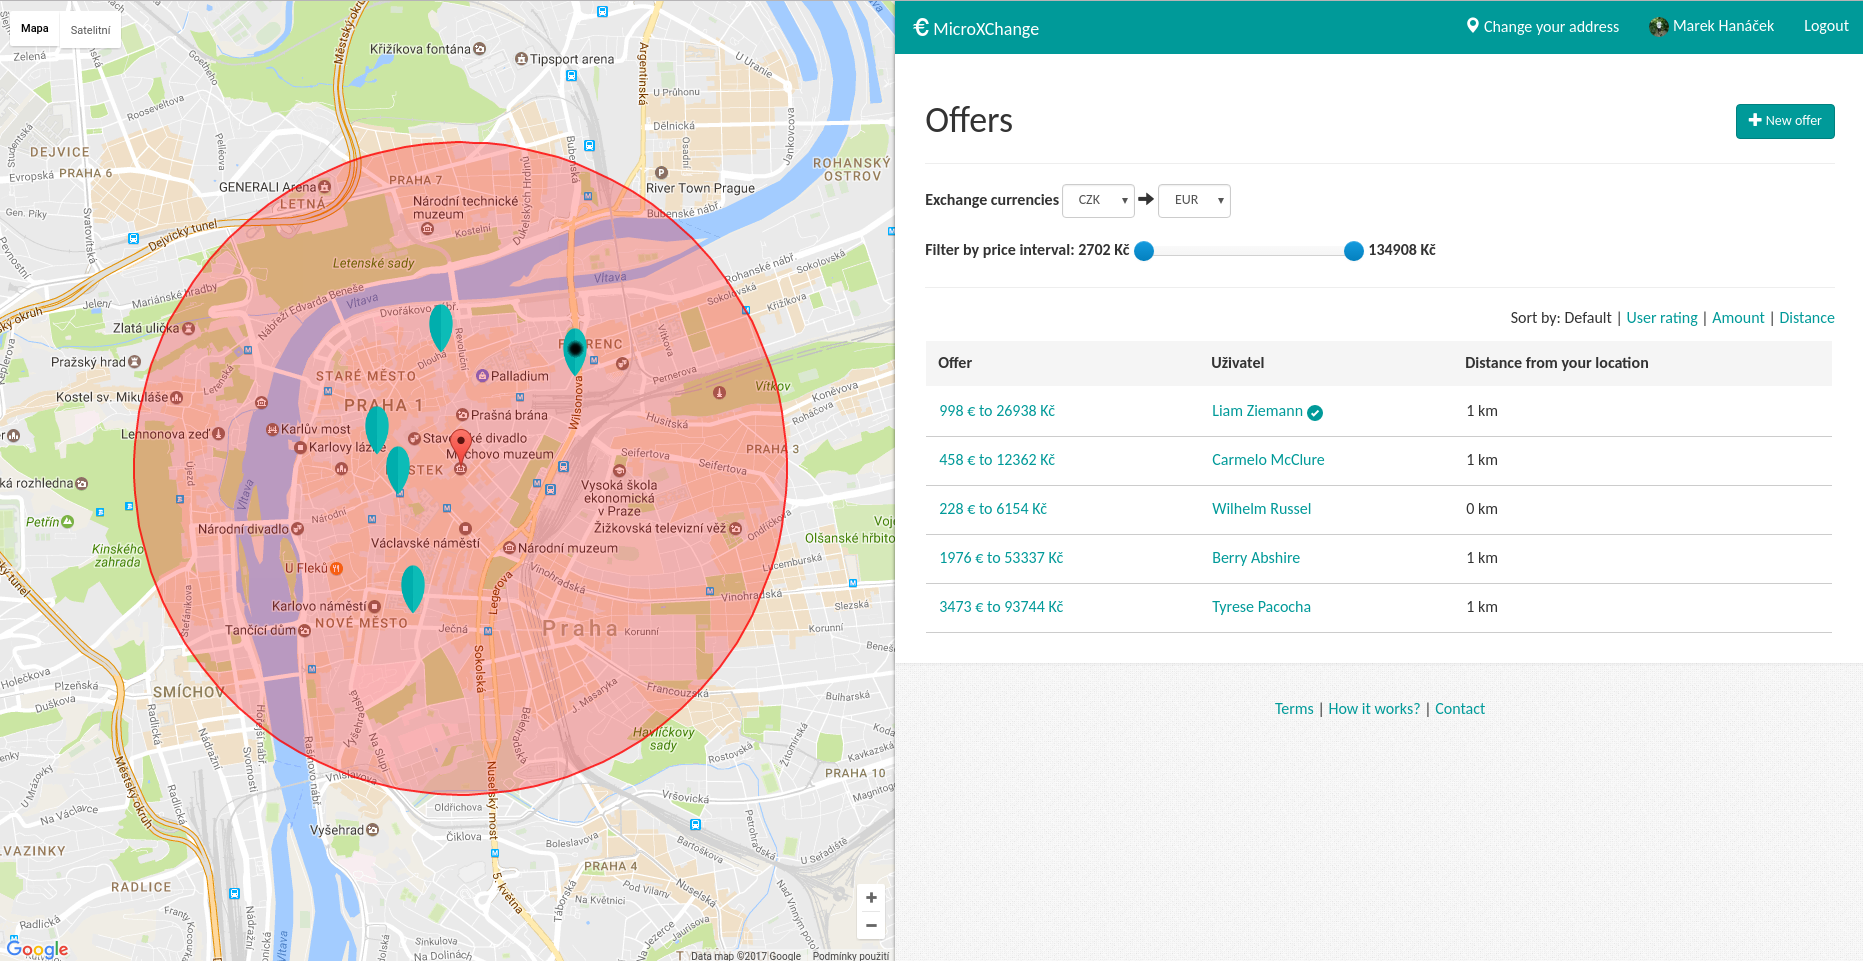
\includegraphics[width=1.0\textwidth]{media/tur/homepage.png}
    \caption{Hlavní stránka aplikace}
    \label{fig:tur:homepage}
\end{figure}

\subsection{Mapa}
Mapa obsahuje ukazatel polohy uživatele, kruh znázorňující vyhledávací rádius a ukazatele poloh nabídek. Ukazatel polohy uživatele a poloh nabídek jsou barevně odlišeny.

\subsection{Textová část}
Textová část se skládá z~hlavičky, filtračního formuláře, seznamu nabídek s~možností seřazení, tlačítka pro vytvoření nové nabídky a patičky obsahující odkazy na informační stránky.

\subsection{Filtrace nabídek}
Formulář obsahuje tři základní parametry, pomocí nichž lze filtrovat:
\begin{itemize}
	\item Měnu, ze které chceme peníze směnit,
	\item měnu, do které chceme peníze směnit,
	\item interval obnosu peněz.
\end{itemize}
Filtrace dále bere v~potaz i aktuální, respektive uživatelem zadanou polohu, a rádius. Filtrace se samozřejmě projevuje i v~mapě. Jsou tedy zobrazeny jen ty nabídky, které odpovídají zadaným filtrům.

\subsection{Řazení nabídek}
Vidno na obrázku \ref{fig:tur:sorting}. Nabídky lze seřadit čtyřmi různými způsoby:
\begin{itemize}
	\item Vzestupně dle vzdálenosti uživatelovy polohy od centra nabídky.
	\item Vzestupně dle obnosu peněz nabídek.
	\item Sestupně dle hodnocení uživatelů.
	\item Dle kombinace více kritérií nabídek. Tento způsob blíže popisuji v~následující podkapitole.
\end{itemize}

\begin{figure}[!h]
    \centering
    
\includegraphics[width=1.0\textwidth]{media/tur/sorting.png}
    \caption{Výpis nabídek s~možností seřazení}
    \label{fig:tur:sorting}
\end{figure}

\subsubsection{Řazení nabídek dle kombinace více kritérií}
Hodnocení se skládá ze dvou složek:
\begin{itemize}
	\item Hodnocení uživatele:
        \begin{itemize}
            \item Jestliže má uživatel měně než dvě hodnocení, pak je tato hodnota rovna 0.
            \item Jestliže má uživatel dvě a více hodnocení, pak se hodnota odvíjí od průměrného počtu hvězdiček. Za špatné hodnocení je penalizován, za dobré hodnocení pak odměněn kladnými body. Konkrétně\footnote{Uvedené hodnocení a penalizace jsou založeny na základě experimentálního zkoumání řazení s~velkým množstvím testovacích dat.}:
            \begin{itemize}
                \item 1 hvězdička $\rightarrow$ penalizace -1.5,
                \item 2 hvězdičky $\rightarrow$ penalizace -1,
                \item 3 hvězdičky $\rightarrow$ hodnocení je rovno 0.6,
                \item 4 hvězdičky $\rightarrow$ hodnocení je rovno 0.8,
                \item 5 hvězdiček $\rightarrow$ hodnocení je rovno 1.
            \end{itemize}
        \end{itemize}
	\item Vzdálenost od uživatele:
        \begin{itemize}
            \item Za vzdálenost od uživatele může nabídka dostat 0 až 1 bod.
            \item Hodnota se počítá na základě vzdálenosti nejbližší a nejvzdálenější nabídky a dále na základě vzdálenosti právě hodnocené nabídky.
            \item Kód výpočtu této hodnoty lze vidět v ukázce kódu \ref{code:sorting-distance}.
            \item Čím blíže je tedy nabídka k~zákazníkovi tím lepší hodnocení obdrží.
            \item \textit{Příklad}: V~případě tři nabídek ve vzdálenostech 15~km, 2~km a 28~km, budou hodnocení 0.5, 1 a 0.
        \end{itemize}
\end{itemize}

\begin{listing}[htbp]
\caption{\label{code:sorting-distance}Funkce pro výpočet hodnocení vzdálenosti od uživatele}
\begin{minted}[frame=lines,bgcolor=codebg,fontsize=\footnotesize,linenos,breaklines]{Python}
def get_distance_rating(offer, min_distance, max_distance, lat, lng):
    """
    Keyword arguments:
    offer -- concrete offer
    min_distance -- distance of nearest offer
    max_distance -- distance of the furthest offer
    lat -- input latitude
    lng -- input longitude
    """
    distance_from_min = get_offer_distance_from(offer, lat, lng) - min_distance
    min_max_distance = max_distance - min_distance
    percent = min_max_distance / 100
    return 1 - ((distance_from_min / percent) / 100)
\end{minted}
\end{listing}

\subsection{Mobilní verze}
Stejně jako při návrhu desktopové verze, tak i při návrhu mobilní verze je návrh inspirován webem Sreality.cz, který byl analyzován v~kapitole \ref{analyza:sreality}. Zobrazuje se tedy vždy pouze mapa nebo textová část. Viz obrázek \ref{fig:tur:homepage-mobile} na straně \pageref{fig:tur:homepage-mobile}.

\begin{figure}[!h]
    \centering
    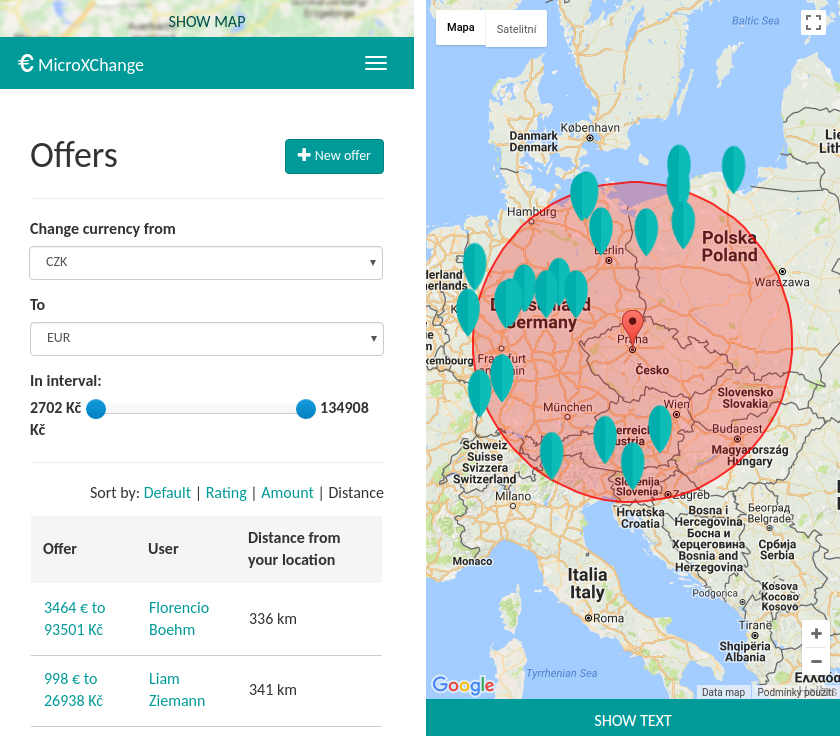
\includegraphics[width=1.0\textwidth]{media/tur/homepage-mobile.png}
    \caption{Mobilní verze aplikace}
    \label{fig:tur:homepage-mobile}
\end{figure}

\section{Detail nabídky}

\label{nur:detail}

Existují 2 verze zobrazení detailu nabídky. A~to zobrazení spolu s~mapou a zobrazení na samostatné stránce.

\subsection{Zobrazení spolu s~mapou}
Tímto způsobem se zobrazují pouze nabídky, které jsou volné\footnote{Status nabídky je \textit{Awaiting acceptance}.}. V~mapě se zobrazuje čára mezi umístěním uživatele a umístěním nabídky. V~textové části pak základní informace o~nabídce a dále také informace o~uživateli. Stránka dále obsahuje tlačítko, které slouží k~projevení zájmu o~danou nabídku. V~případě, že již uživatel má nějaké zkušenosti s~tímto uživatelem, jsou zobrazeny jejich společné nabídky. Z~detailu nabídky se lze vrátit zpět na výpis nabídek pomocí tlačítka \textit{Zpět} (Back). Detail nabídky lze vidět na obrázku \ref{fig:tur:offer-detail-map}.

\begin{figure}[!h]
    \centering
    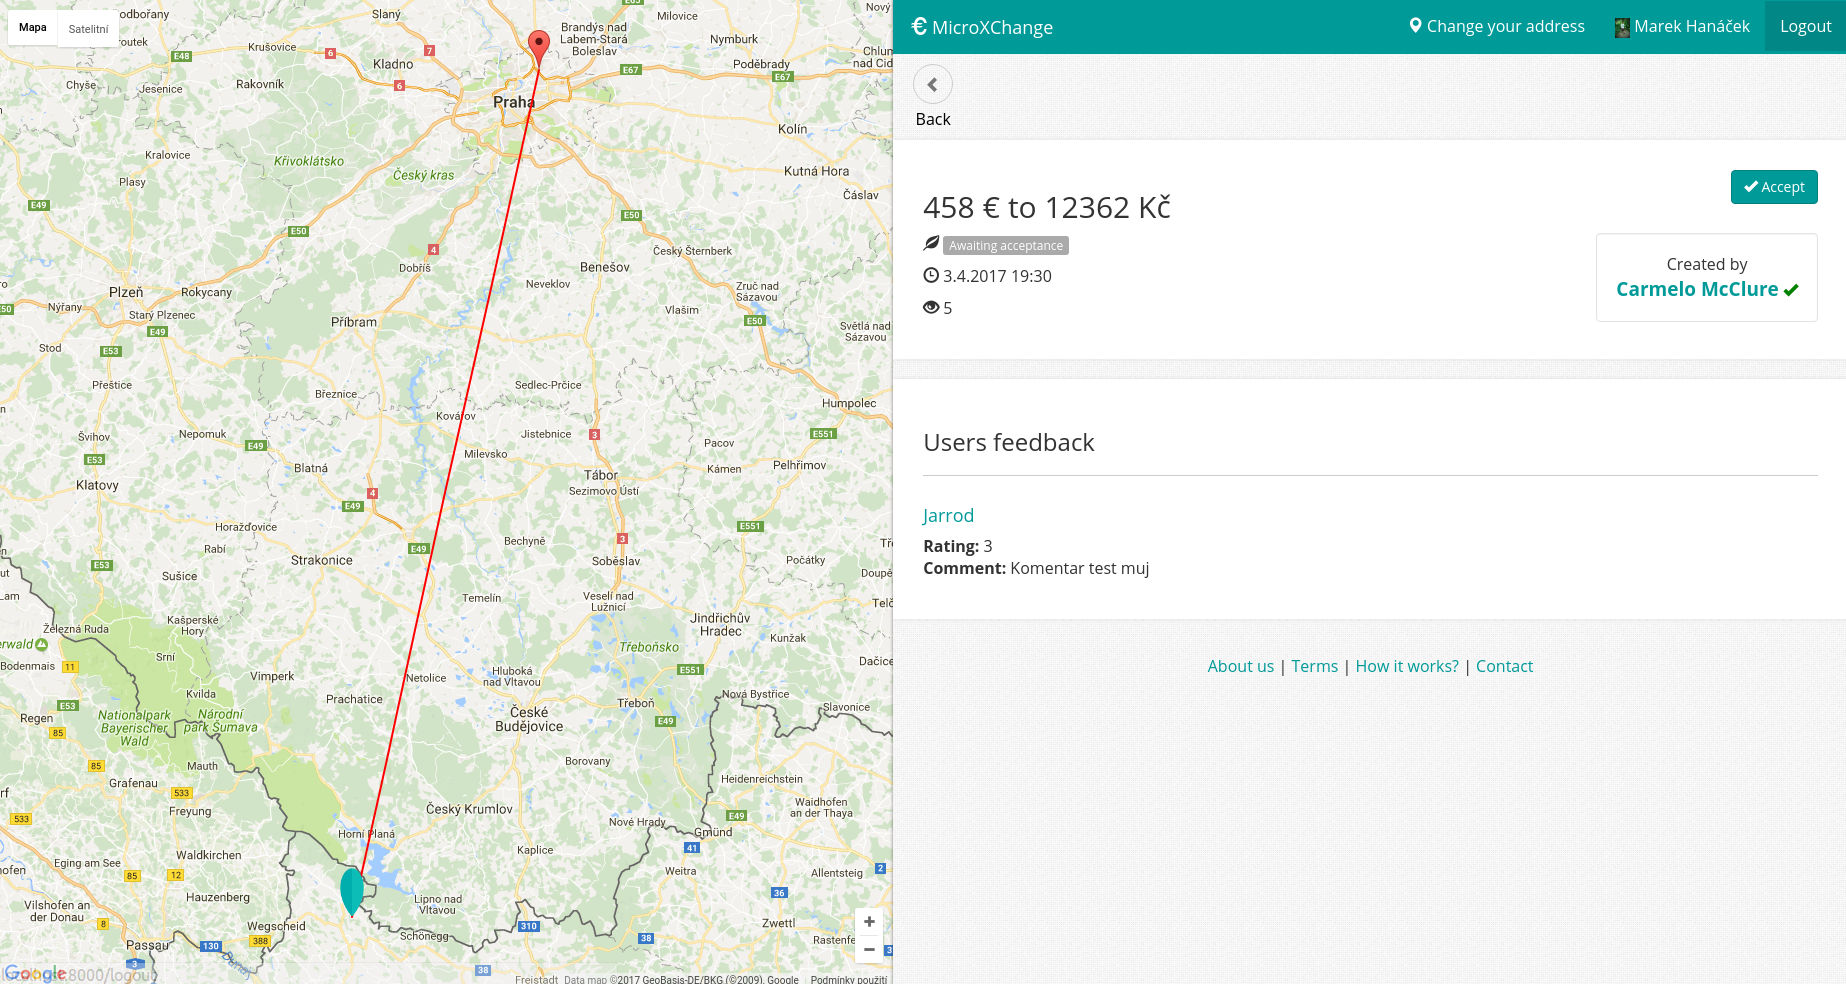
\includegraphics[width=1.0\textwidth]{media/tur/offer-detail-map.png}
    \caption{Detail nabídky s~mapou}
    \label{fig:tur:offer-detail-map}
\end{figure}

\subsection{Zobrazení na samostatné stránce}
Zobrazení je dostupné pouze v~případě, že uživatel je přiřazen k~nabídce. Toto zobrazení obsahuje totožné informace jako zobrazení s~mapou. Při rozvržení bez mapy však máme více prostoru a detail nabídky je tedy uspořádán jinak. Na toto zobrazení se uživatel dostane ze svého uživatelského profilu. Detail nabídky s~tímto rozvržením lze vidět na obrázku \ref{fig:tur:offer-detail-no-map} na straně \pageref{fig:tur:offer-detail-no-map}.

\begin{figure}[!h]
    \centering
    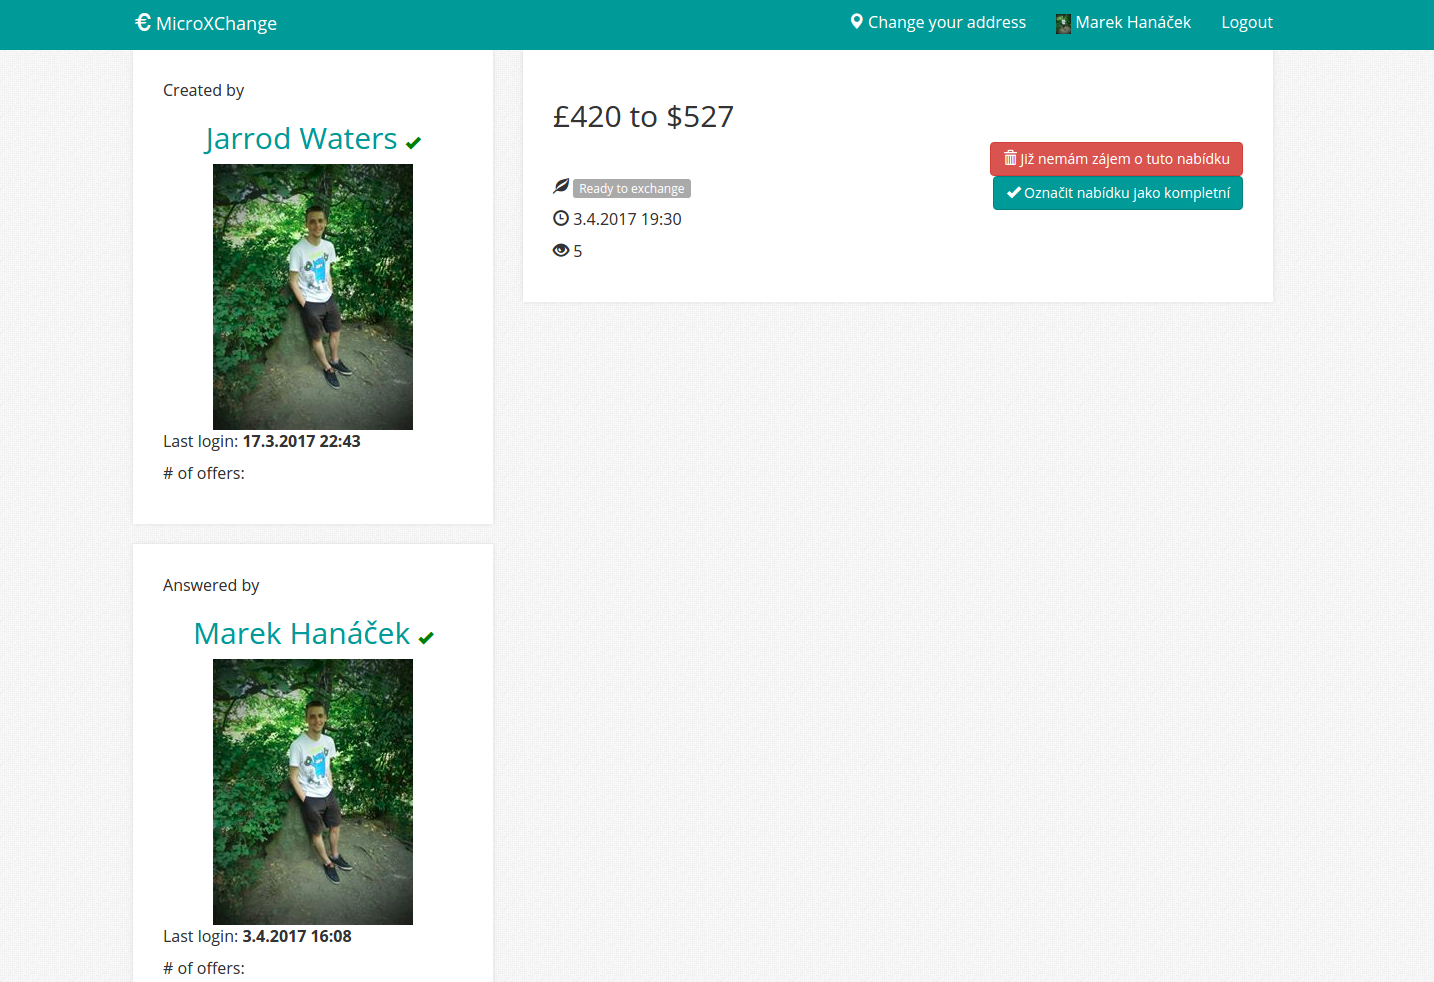
\includegraphics[width=1.0\textwidth]{media/tur/offer-detail-no-map.png}
    \caption{Detail nabídky bez mapy}
    \label{fig:tur:offer-detail-no-map}
\end{figure}
\section{Můj profil}
\label{nur:my-profile}

Stránka \textit{Můj profil} obsahuje základní informace o~uživateli, jako je jeho aktuální adresa, rádius a hodnocení uživatele.
Profil uživatele zobrazuje všechny aktuální nabídky, které jsou dále rozděleny na sekce dle toho, zda daná nabídka čeká na akci právě přihlášeného uživatele nebo na akci někoho jiného. Další sekcí jsou již dokončené nabídky s~přehledem hodnocení, případně s~odkazem na přidání hodnocení. Podoba stránky je na obrázku \ref{fig:tur:my-profile} na straně \pageref{fig:tur:my-profile}.

\begin{figure}[!h]
    \centering
    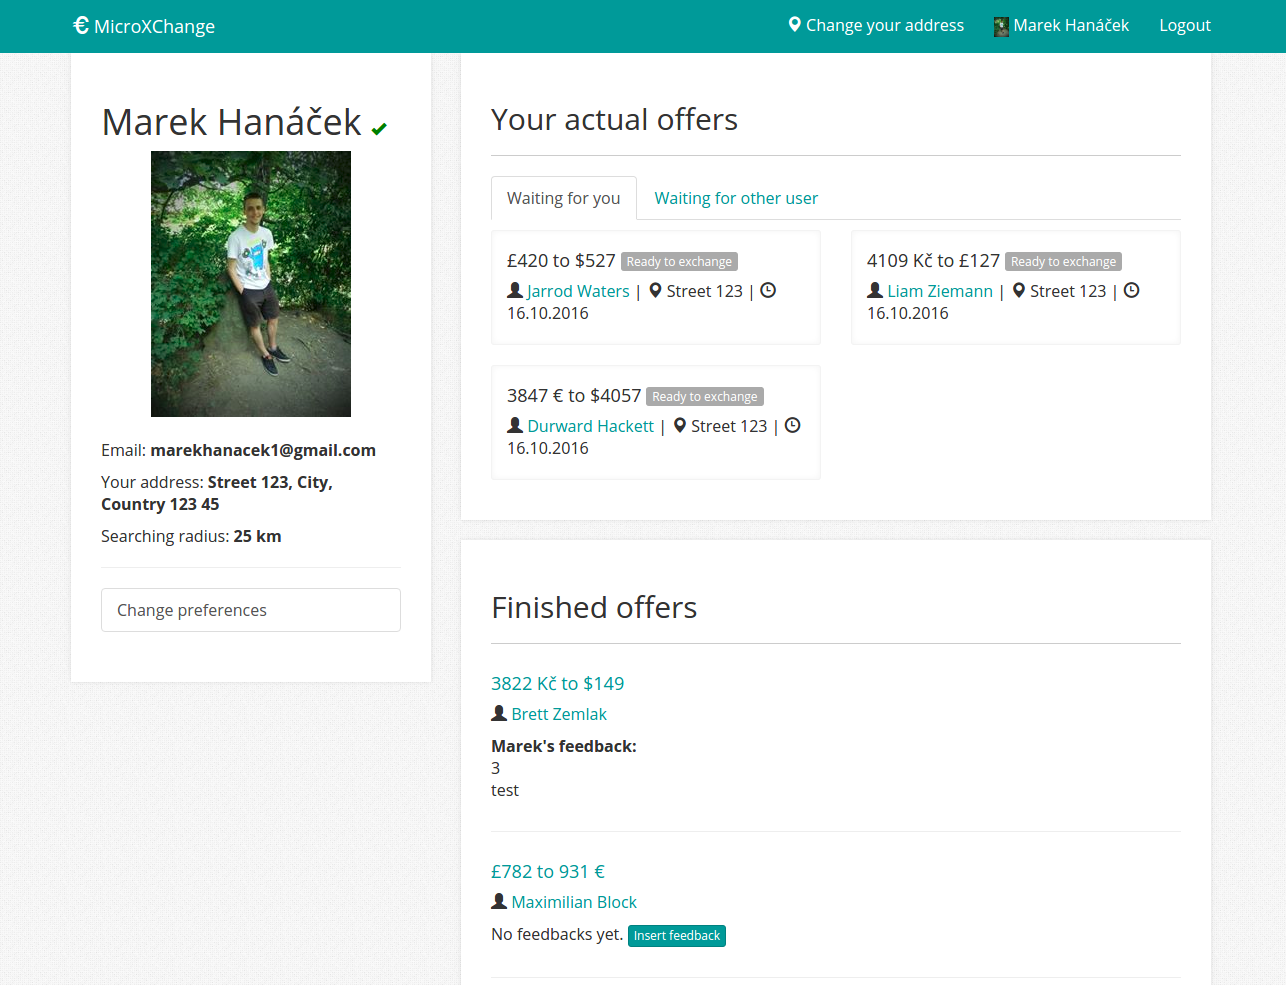
\includegraphics[width=1.0\textwidth]{media/tur/my-profile.png}
    \caption{Můj profil}
    \label{fig:tur:my-profile}
\end{figure}
\section{Profil uživatele}

\label{nur:user-profile}

Obsahuje základní informace o uživateli, jeho hodnocení a nabídky které má aktuálně přihlášený uživatel s daným uživatelem společné. Rozvržení je velmi podobné podstránce \textit{Můj profil}. Podoba stránky je na obrázku \ref{fig:tur:user-profile}.

\begin{figure}[h]
    \centering
    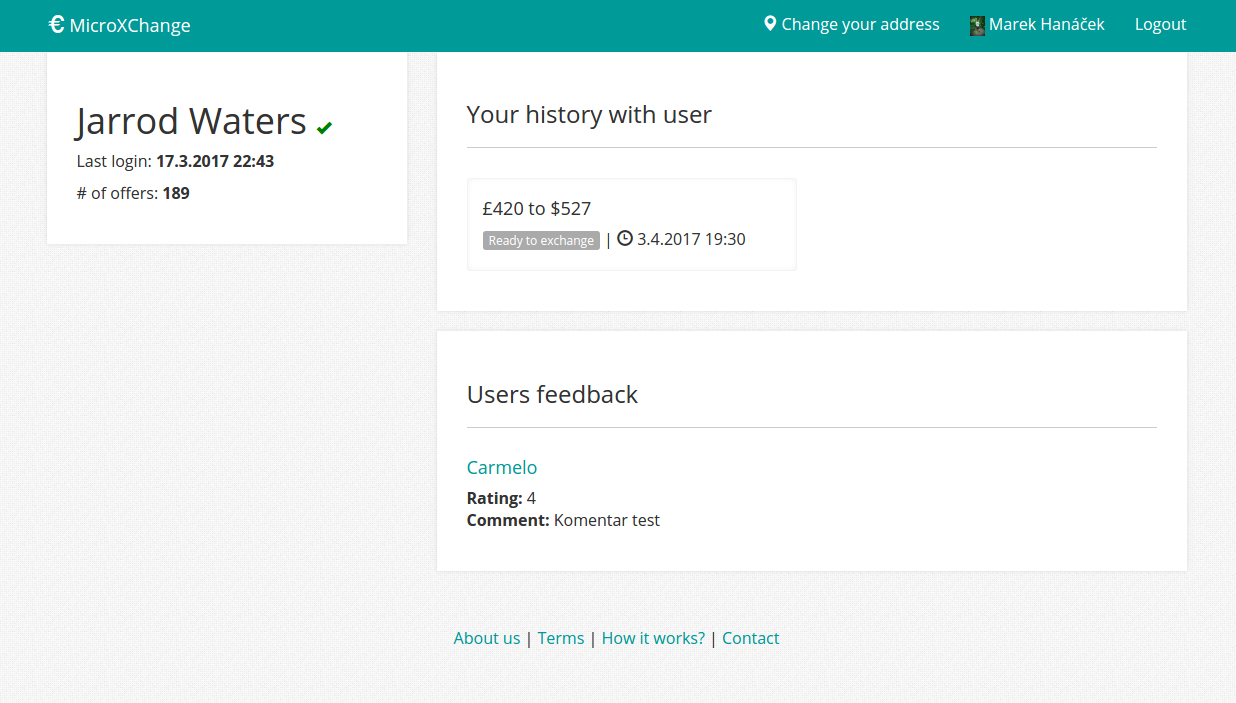
\includegraphics[width=1.0\textwidth]{media/tur/user-profile.png}
    \caption{Profil uživatele}
    \label{fig:tur:user-profile}
\end{figure}
\section{Nová nabídka}

\label{nur:new-offer}

Viz obrázek \ref{fig:tur:new-offer} na straně \pageref{fig:tur:new-offer}. Pokud uživatel nenajde nabídku, která mu vyhovuje, může použít právě tuto stránku, pomocí které vytvoří novou. Formulář pro přidání nové nabídky obsahuje:
\begin{itemize}
    \item Měny, které budou směněny,
    \item částky v~jednotlivých měnách,
	\item adresu,
	\item poloměr,
	\item komentář k~nabídce,
	\item mapu -- Pro lepší orientaci při zadávání adresy a poloměru je v~pravé části stránky umístěna mapa, která zobrazuje aktuální výběr adresy a poloměr pro vyhledávání.
\end{itemize}

\begin{figure}[!h]
    \centering
    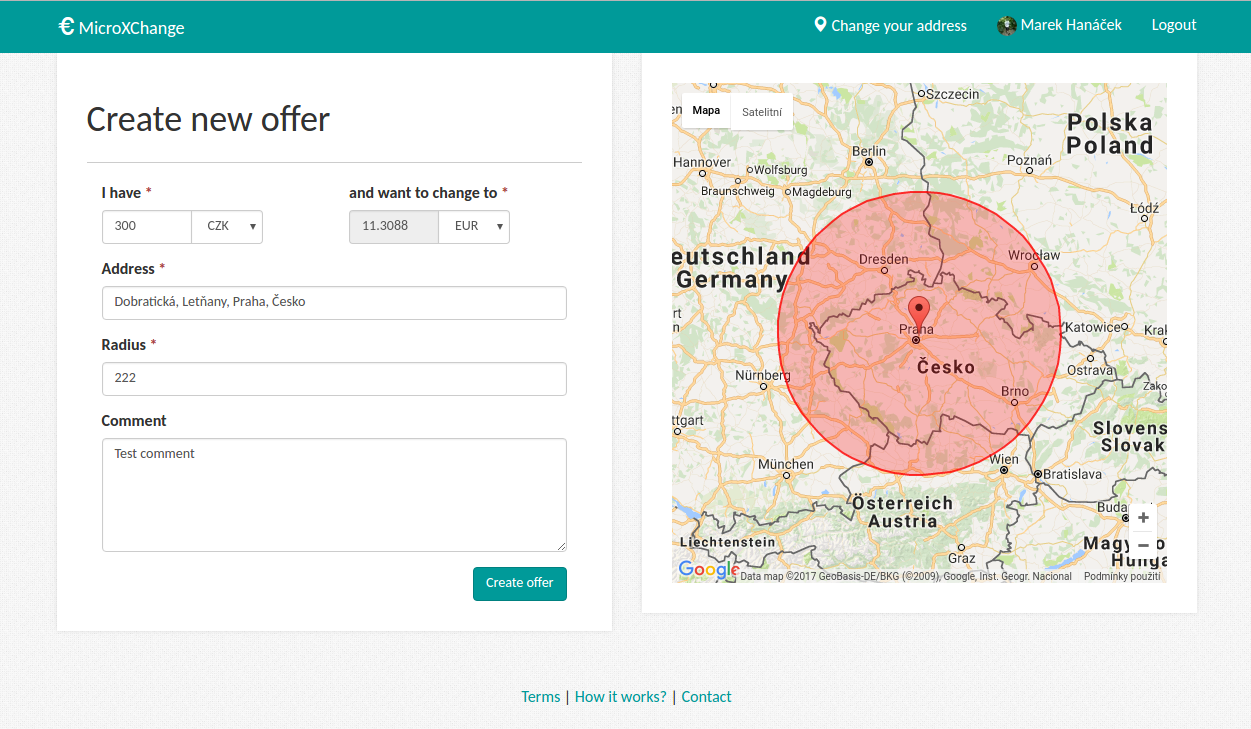
\includegraphics[width=1.0\textwidth]{media/tur/new-offer.png}
    \caption{Nová nabídka}
    \label{fig:tur:new-offer}
\end{figure}
\section{Ostatní sekce}
\label{nur:other-sections}

Všechny informativní stránky mají velmi podobné rozvržení, které je vidět na obrázku \ref{fig:tur:contact}.

Mezi ostatní stránky patří:
\begin{itemize}
    \item \textbf{Terms} - Informativní stránka s podmínkami užití.
    \item \textbf{Jak to funguje?} - Obsahuje krátký popis toho, k čemu stránka slouží a jak ji používat.
    \item \textbf{Kontakty} - Obsahuje kontaktní informace pro případně připomínky uživatelů.
\end{itemize}

\begin{figure}[h]
    \centering
    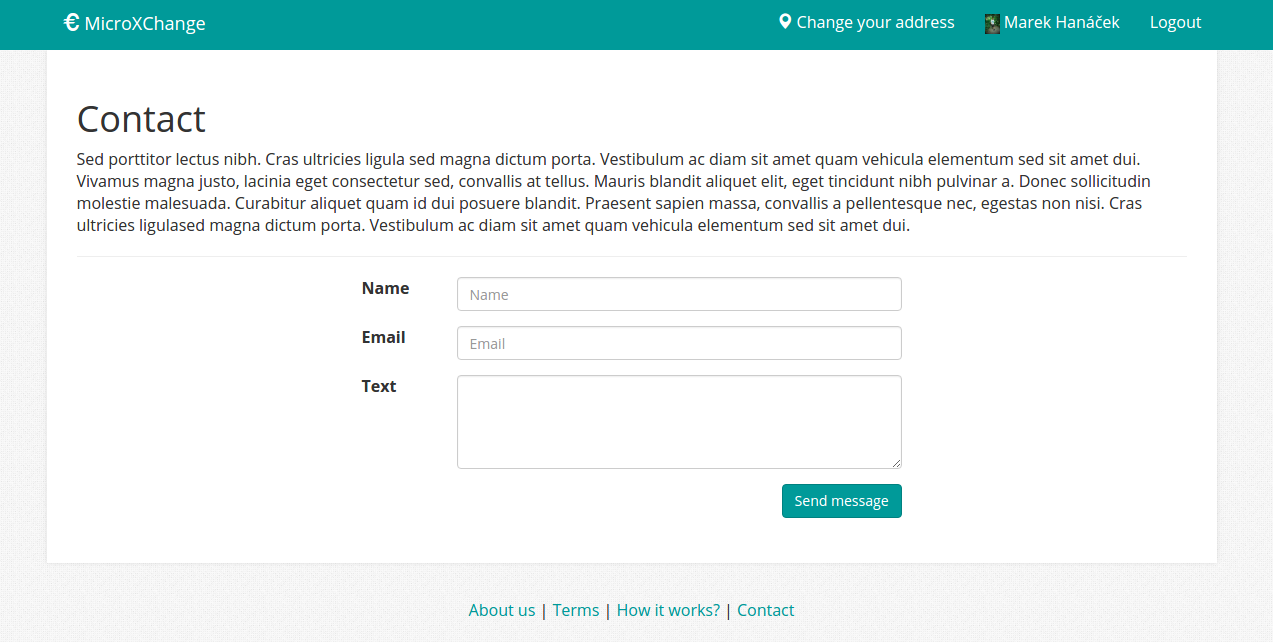
\includegraphics[width=1.0\textwidth]{media/tur/contact.png}
    \caption{Informační stránka Kontakty}
    \label{fig:tur:contact}
\end{figure}
\section{Hodnocení uživatelů}
\label{nur:feedback}

TODO
\section{Změna adresy}

\label{nur:address-change}

Změnu adresy lze provést dvěma způsoby: přes uživatelský profil nebo přímo tlačítkem \textbf{Změnit adresu} (Change your address). Po použití tohoto tlačítka se zobrazí modální okno (obrázek \ref{fig:tur:address-change} na straně \pageref{fig:tur:address-change}), kde si uživatel zadá svou polohu (zadáním adresy nebo pomocí tlačítka moje poloha) a zvolí rádius pro vyhledávání. Poté pomocí tlačítka \textbf{Uložit} (Save) adresu uloží.

\begin{figure}[!h]
    \centering
    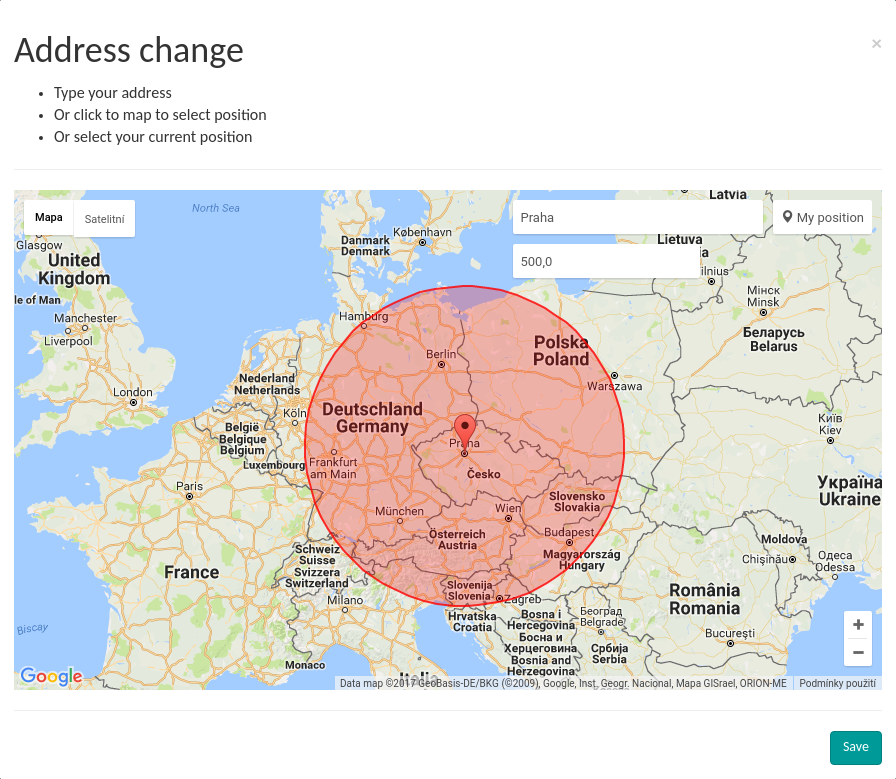
\includegraphics[width=1.0\textwidth]{media/tur/address-change.png}
    \caption{Změna adresy}
    \label{fig:tur:address-change}
\end{figure}
\section{Heuristická analýza}

\label{nur:test}

Testování uživatelského rozhraní je prováděno pomocí heuristické analýzy. Heuristická analýza obsahuje 10 bodů, které by mělo splňovat každé uživatelské rozhraní. Jak udává zdroj [7], jsou to tyto:

\begin{enumerate}
    \item Viditelnost stavu systému:
        \begin{itemize}
            \item Systém nesmí zůstat zamrzlý a nereagovat na uživatelské vstupy.
            \item Zobrazit ukazatel průběhu.
            \item Uživatel musí být informován o~tom, co systém dělá.
        \end{itemize}
    \item Shoda mezi systémem a realitou:
        \begin{itemize}
            \item Zachováni konvencí (a metafor) reálného světa.
            \item Ikony (a metafory) se musí chovat jako to, co zobrazují / na co odkazují.
            \item Do koše mohu věci nejen vyhodit, ale lze ho i vysypat, případně ho prohledat a vytáhnout už jednou vyhozenou věc.
            \item Pozor na překlady.
        \end{itemize}
    \item Minimální zodpovědnost (a stres):
        \begin{itemize}
            \item Nic se nemůže pokazit.
            \item Vždy je možnost vrátit se zpět do předchozího stavu.
            \item Uživatelé více experimentují a rychleji se učí.
            \item Uživatel ovládá systém, ne naopak.
            \item Zrušení dlouho trvajících operací.
            \item Potvrzování akcí.
            \item Varováni před provedením nevratné akce.
        \end{itemize}
    \item Shoda s~použitou platformou a obecnými standardy:
        \begin{itemize}
            \item Program pod Windows vypadá a chová se jako pod Windows. Nijak jinak.
            \item Pokud to jde, použít standardní systémové komponenty.
            \item Systémové barvy a typy písem.
            \item Používat stejné termíny.
            \item Vysvětlit zkratky.
        \end{itemize}
    \item Prevence chyb:
        \begin{itemize}
            \item Uživatel by neměl mít možnost zadat špatnou hodnotu.
            \item Následná chybová hláška to zachrání jen částečně.
            \item Pokud je způsob zadáváni z~principu složitější, je třeba to na místě vysvětlit.
            \item Zvýraznit povinné položky formulářů.
            \item Potvrzování akcí.
        \end{itemize}
    \item Kouknu a vidím:
        \begin{itemize}
            \item Nezatěžovat uživatelovu paměť.
            \item Akce, které uživatel může momentálně provést by měly být viditelné a snadno dosažitelné.
            \item Stejně tak informace.
            \item Nepotřebné kontrolky a informace nepotřebujeme.
            \item Pozice uživatele.
            \item Pozice ve stromové struktuře.
        \end{itemize}
    \item Flexibilita a efektivita:
        \begin{itemize}
            \item Zkušení vs. běžní uživatelé.
            \item To co zkušený uživatel pravidelně potřebuje, běžný kolikrát ani nepotřebuje vědět.
            \item Pokročilý mód.
            \item Klávesové zkratky / funkční klávesy.
            \item Makra.
            \item Klonování existujících záznamů.
            \item Jsou opravdu všechny akce/nastavení potřeba?
        \end{itemize}
    \item Minimalita (Klapky na očích):
        \begin{itemize}
            \item Zobrazovat pouze informaci, která aktuálně k~něčemu opravdu je.
            \item Čim méně možností uživatel má, tím rychleji koná.
            \item (Nepotřebná) grafika by neměla zastiňovat ovládání a účel.
            \item Cokoliv je zobrazeno soutěží o~uživatelovu pozornost.
            \item Je třeba nechat vyhrát to důležité.
        \end{itemize}
    \item Smysluplné chybové hlášky:
        \begin{itemize}
            \item Nejlepší je nedojít do stavu kdy je třeba chybového hlášení.
            \item Chybové hlášení v~běžném jazyce – žádné kódy.
            \item Chybové hlášení by mělo popsat co se stalo špatně, jak se to stalo a jak tomu příště předejít.
            \item Případně možná řešení doporučit.
            \item Mělo by poučit (vzdělat) uživatele.
        \end{itemize}
    \item Pomoc a dokumentace:
        \begin{itemize}
            \item Systém by měl být použitelný bez jakékoliv nápovědy, nicméně nápověda musí být.
            \item Musí podporovat funkci vyhledávání.
            \item Spíše než popisem by se měla zabývat příklady.
            \item Kontextová nápověda.
        \end{itemize}
\end{enumerate}

\subsection{Nalezené problémy}
Nalezené problémy jsou shrnuty v~tabulce \ref{tab:heuristic-analysis}. Každý z~nalezených problémů je hodnocen na stupnici 1 - 5, kde 1 znamená málo závažný problém a oproti tomu 5 značí velmi závažný problém. Pro všechny nalezené problémy je také navržen způsob řešení vedoucí k~odstranění problému. Všechny nalezené problémy byly před dalším vývojem aplikace vyřešeny.

\begin{table}[!h]
    \caption{Problémy nalezené při heuristické analýze}\label{tab:heuristic-analysis}
    \begin{tabulary}{1.0\textwidth}{|L|L|L|L|}
        \hline
        Bod analýzy & Nalezený problém & Závažnost problému (1 -- 5) & Řešení problému \\ \hline\hline
        4. & Sjednotit výrazy \textit{offer} a \textit{transaction}. & 2 & V~rámci celého webu se nyní používá výraz \textit{offer}. \\ \hline
        5. & Nejsou zvýrazněny povinné položky formulářů. & 3 & Byla přidána červená * k~povinným položkám formulářů. \\ \hline
        6. & Nelze rozpoznat, podle čeho se řadí. & 4 & Byl odstraněn odkaz z~aktuálního řazení. Došlo tak k~barevnému odlišení textů. \\ \hline
        10. & Chybí nápověda o~postupu práce s~nabídkou. & 4 & Byla přidána stránka \textit{Jak to funguje?} s~popisem a stavovým diagramem transakce. \\ \hline
    \end{tabulary}
\end{table}



